\section{\Y{geometry}により簡単にページ設定を行う}
\zindind{版面}{の設定}%
\indindz{余白}{上下左右の}%

\Y{geometry}はページ設定を簡単に行えるパッケージです.
\begin{usage}
 \usepackage[$\<ページ設定>$]{geometry}
 \geometry{$\<ページ設定>$}
\end{usage}
\cmd{usepackage}で読み込むときのオプションで\val{ページ設定}の設定を
する事も可能ですし,\sty{geometry}パッケージを読み込んだ後に \C{geometry}
コマンドで設定する事もできます(\cmd{geometry}コマンドはプリアンブルでの
み使う事が出来ます).

次のようにすると文章領域の上下左右の余白を 2\,cmに設定します(用紙にはヘッ
ダ,フッタ,傍注がありますから,これらの領域を除いた文面の余白が 2\,cmと
いう事になります).
\begin{intext}
\usepackage[margin=2cm]{geometry} 
\end{intext}

\sty{jsclasses}に含まれる\Cls{jsbook}を用いている場合は以下の1行を
入れると正しくページ設定できる場合があります.
\begin{intext}
\setlength\fullwidth{\textwidth}
\end{intext}

\subsection{用紙の各部の名称}

\begin{figure}[htbp]
 \begin{center}
  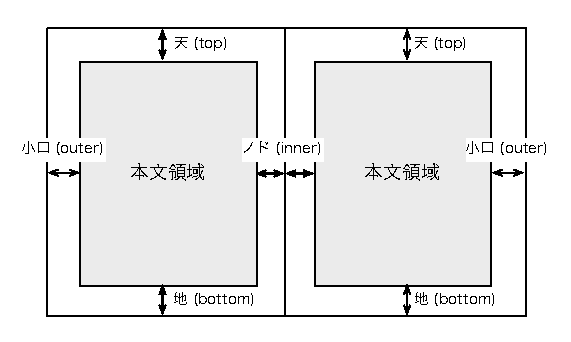
\includegraphics{name}
  \caption{片面印刷時の用紙各部の名称}
 \end{center}
\end{figure}

\begin{figure}[htbp]
 \begin{center}
  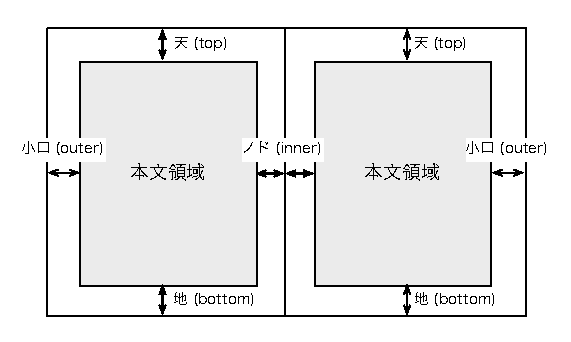
\includegraphics{name}
  \caption{両面印刷時の用紙各部の名称}
 \end{center}
\end{figure}


%オプションについては後述しますが,本書も\sty{geometry}パッケージを用いて,
%次のようにページ設定されています.

%\begin{intext}
%\usepackage[%showframe,% for debug
%  paperwidth=128mm,paperheight=182mm,% JIS B6
%  outer=15mm,inner=15mm,% 小口 = outer, ノド = inner
%  tmargin=16mm,bmargin=15mm,% 天 = tmargin, 地 = bmargin
%  headsep=.5\cvs,% 柱と本文の空き
%  ignorefoot,ignoremp]{geometry}% フッター・傍注は無視
%\end{intext}

\subsection{デバイスドライバを指定する}

\begin{description}
 \item[\Option{dvips}] \Prog{dvips}用に用紙サイズ情報を設定します.
 \item[\Option{dvipdfm}] \Prog[dvipdfm]{\Dvipdfm}用に用紙サイズ情報を設
 定します.
 \item[\Option{pdftex}] \Prog[pdftex]{\PDFTeX},
 \Prog[pdflatex]{\PDFLaTeX}用に用紙サイズ情報を設定します.
\end{description}

\subsection{デバッグ情報を表示する}
\begin{description}
 \item[\Option{verbose}] 
  \Y{geometry}パッケージの処理内容を詳細に表示します.
 \item[\Option{showframe}] 
  ページレイアウトの設定を確認するために,1ページ目の本文領域,ヘッダー,
  フッターを枠で囲みます.
\end{description}


\subsection{用紙サイズを指定する}
\begin{usage}
\geometry{$\<既定のサイズ>$}
\geometry{papersize=$\<用紙の幅>$,$\<用紙の高さ>$}
\geometry{paperwidth=$\<用紙の幅>$}
\geometry{paperheight=$\<用紙の高さ>$}
\end{usage}

\val{既定のサイズ}には以下のオプションがあります.
\begin{description}
 \item[既定のサイズ]
\zindind{用紙}{の既定のサイズ}
  \Optionlist{a0paper,a1paper,a2paper,a3paper,a4paper,a5paper,a6paper,%
  b0paper,b1paper,b2paper,b3paper,b4paper,b5paper,b6paper,%
  letterpaper,executivepaper,legalpaper,screen}.
  \option{screen} は 225\,mm $\times$ 180\,mm になります.
  \option{screen}は\option{centering} も併用すると便利です.
  `\str{paper=}\val{用紙サイズ}'と記述しても大丈夫です.
    ただし,B列の用紙はJISではなくISOのサイズであるため,JISのB5にしたけ
    れば,直接以下の\option{papersize}オプションを使って
    \verb|papersize={182mm,257mm}| とする必要があります.
\item[\Option{paperwidth}] 
\zindind{用紙}{の幅}
  \Z{用紙}の幅を,\val{長さ}を指定して決めます.
  `\str{paperwidth=10cm}'のように使います.
\item[\Option{paperheight}]
\zindind{用紙}{の高さ}
  用紙の高さを,\val{長さ}を指定して決めます.
\item[\Option{papersize}]
  `\option{papersize}\str=\twoargs{幅}{高さ}'とするか,
  `\option{papersize}\str=\val{長さ}'とすれば \option{paperwidth}
  と\option{paperheight}を用いた事と等価になります.
\end{description}

%JIS~B6にする.
%\begin{intext}
%\usepackage[paperwidth=128mm,paperheight=182mm]{geometry}
%\end{intext}

\subsection{用紙の方向を指定する}
\begin{description}
\item[\Option{landscape}] 
  \Z{横置き}でページレイアウトを設定します.
\item[\Option{portrait}]
  \Z{縦置き}でページレイアウトを設定します.
\end{description}


\subsection{紙面で本文領域が占める割合を指定する}

\begin{description}
 \item[\Option{hscale}] 
  用紙の幅 (\C{paperwidth}) に対して本文領域が占める横幅の比率です.
  `\str{hscale=.8}' とすると `\str{width=.8\BS paperwidth}' と等価になりま
  す.標準は 0.7 です.
 \item[\Option{vscale}] 
  用紙の高さ (\C{paperheight}) に対して本文領域が占める高さの比率です.
  `\str{vscale=.8}' とすると `\str{height=.9\BS paperheight}' と等価になりま
  す.標準は 0.7 です.
 \item[\Option{scale}] 
  本文が幅と高さに関して用紙に対して占める比率を指定します.
  `\str{scale=}\twoargs{幅の比率}{高さの比率}'
   とするか`\str{scale=}\val{比率}'として使います.標準は 0.7 です.
\end{description}

\subsection{本文領域の幅・高さの長さを直接指定する}
\begin{description}
 \item[\Option{width}/\Option{totalwidth}] 
\indindz{幅}{本文のトータルな}
  本文のトータルな幅を指定します.`\str{width=}\val{長さ}'とするか,
  `\str{totalwidth=}\val{長さ}'とします.
 \item[\Option{height}/\Option{totalheight}] 
\indindz{高さ}{本文のトータルな}
  本文のトータルな高さを指定します.`\str{height=}\val{長さ}'とするか,
  `\str{totalheight=}\val{長さ}'とします.
 \item[\Option{total}] 
  本文のトータルな幅と高さを指定します.
  `\str{total=}\twoargs{幅}{高さ}'とするか,
  `\str{total=}\val{長さ}'とします.
 \item[\Option{textwidth}] 
   文章領域となる \C{textwidth} の幅を指定します.
   `\str{textwidth=}\val{長さ}'とします.
 \item[\Option{textheight}]
   文章領域となる \C{textheight} の高さを指定します.
   `\str{textheight=}\val{長さ}'とします.
 \item[\Option{text}/\Option{body}]
  \C{textwidth} と \C{textheight} の両方を指定します.
  `\str{body=}\twoargs{幅}{高さ}'とするか`\str{text=}\val{長さ}'とします.
\end{description}



\subsection{1行の文字数を指定する}
\begin{usage}
\geometry{textwidth=$\<文字数>$zw}
\end{usage}

\subsection{本文の高さを行送りの倍数にする}

%\begin{usage}
%\setlength{\baselineskip}{$\<行の高さ>$} 
%\end{usage}

\begin{description}
  \item[\Option{heightrounded}]
  本文の高さが行送りの倍数でない場合に,``\str{underfull vbox}''の警告を
  出さないように \C{textheight} を \val{\C{baselineskip} の整数倍 $+$
  \C{topskip}} にします.
\end{description}

\subsection{1ページの行数を指定して本文の高さを決める}
%\begin{usage}
%\setlength{\textheight}{$\<行数>$\baselineskip} 
%\end{usage}
%しかし,
%\begin{intext}
%\advance\textheight\topskip
%\end{intext}
%しないと適切に処理されない.

\begin{usage}
\usepackage{geometry}
\geometry{lines=$\<行数>$} 
\end{usage}

\begin{description}
 \item[\Option{lines}]
  \cmd{textheight} を\Z{行数}によって決めます.`\str{lines=}\val{整数}'で指定
  します.
\end{description}

\subsection{ヘッダ・フッタ領域を本文の高さに含める/含めない}

\begin{description}
 \item[\Option{includehead}]
  トータルな本文の高さ\option{height}/\option{totalheight}にヘッダー
  (\C{headheight} と \C{headsep}) を含めるようにします.標準では無効です.
 \item[\Option{includefoot}]
  トータルな本文の高さ\option{height}/\option{totalheight}にフッター
  (\C{footskip}) を含めるようにします.標準では無効です.
 \item[\Option{includeheadfoot}]
  \option{includehead} と \option{includefoot} の両方を有効にします.
\end{description}

\begin{description}
 \item[\Option{ignorehead}]
  トータルな本文の高さにヘッダーを含めないようにします.標準で有効です.
  `\str{includehead=false}'とするのと等価です.
 \item[\Option{ignorefoot}]
  トータルな本文の高さにフッターを含めないようにします.標準で有効です.
  `\str{includefoot=false}'とするのと等価です.
 \item[\Option{ignoreheadfoot}]
  \option{ignorehead} と \option{ignorefoot} の両方を指定した事と等価で
  す.
\end{description}

\subsection{傍注領域を本文の幅に含める/含めない}

\begin{description}
 \item[\Option{includemp}]
  トータルな本文の幅に\Z{傍注} (\C{marginparwidth} と \C{marginparsep}) も
  含めるようにします.\Option{marginparwidth}と\Option{marginparsep}オプ
  ションに依存しています.標準では無効です.
 \item[\Option{ignoremp}]
  トータルな本文の幅に傍注を含めないようにします.標準で有効です.
\end{description}

\subsection{ヘッダ・フッタ・傍注領域を本文領域に含める/含めない}

\begin{description}
  \item[\Option{includeall}]
  \option{includeheadfoot} と \option{includemp} の両方を指定した事と等
  価です.
 \item[\Option{ignoreall}]
  \option{ignoreheadfoot} と \option{ignoremp} の両方を指定した事と等価
  です.
\end{description}


\subsection{本文領域と余白の長さを直接指定する}

\begin{description}
 \item[\Option{hdivide}]
  左余白,文章の幅,右余白を指定します.`\str{hdivide=}%
  \threeargs{左余白}{文章幅}{右余白}'のように使います.
  このオプションは三つのうち二つだけ明確な時に,不定の一つを星`\str{*}'
  に置き換えて`\verb|hdivide={2cm,15cm,*}|'とできます.
 \item[\Option{vdivide}]
  \Z{上余白},文章の高さ,\Z{下余白}を指定します.`\str{vdivide=}%
  \threeargs{上余白}{文章幅}{下余白}'のように使います.
 \item[\Option{divide}]
  `\str{divide=}\threeargs{長さ\mbox{$_1$}}{長さ\mbox{$_2$}}{長さ
  \mbox{$_3$}}'とすると`\str{hdivide=}\threeargs{長さ\mbox{$_1$}}{長さ
  \mbox{$_2$}}{長さ\mbox{$_3$}}'と\str{vdivide=}\threeargs{長さ
  \mbox{$_1$}}{長さ\mbox{$_2$}}{長さ\mbox{$_3$}}'を指定した事と等価にな
  ります.
\end{description}


\subsection{余白の長さ指定する}

\begin{description}
 \item[\Option{left}/\Option{lmargin}/\Option{inner}]
 \zindind{用紙}{の左端}
 用紙の左端と本文領域(版面)とのあいだにある左余白を指定します.
 `\str{lmargin=}\val{長さ}'のように使います.両面印刷指定
 (\Option{twoside}) の場合は\Z{ノド}の長さを設定します.
 \item[\Option{right}/\Option{rmargin}/\Option{outer}]
 \zindind{用紙}{の右端}
 用紙の右端と本文領域とのあいだにある右余白を指定します.
 `\str{rmargin=}\val{長さ}'のように使います.両面印刷指定
 (\Option{twoside}) の場合は\Z{小口}の長さを設定します.
 \item[\Option{top}/\Option{tmargin}]
  用紙の上端と本文領域のとのあいだ(\Z{天})にある上余白を指定します.
 `\str{tmargin=}\val{長さ}'のように使います.
 \item[\Option{bottom}/\Option{bmargin}]
  用紙の下端と本文領域のとのあいだ(\Z{地})にある下余白を指定します.
 `\str{bmargin=}\val{長さ}'のように使います.
 \item[\Option{hmargin}]
  左右余白を指定します.`\str{hmargin=}\twoargs{左余白}{右余白}'とするか,
  `\str{hmargin=}\val{長さ}'とします.
 \item[\Option{vmargin}]
  上下余白を指定します.`\str{vmargin=}\twoargs{上余白}{下余白}'とするか,
  `\str{vmargin=}\val{長さ}'とします.
 \item[\Option{margin}]
  `\str{margin=}\twoargs{長さ\mbox{$_1$}}{長さ\mbox{$_2$}}'とすると,
  `\str{hmargin=}\twoargs{長さ\mbox{$_1$}}{長さ\mbox{$_2$}}'と
  `\str{vmargin=}\twoargs{長さ\mbox{$_1$}}{長さ\mbox{$_2$}}'を指定した
  事と等価になります.
\end{description}

\subsection{余白の比率を指定する}

\begin{description}
 \item[\Option{hmarginratio}]
  左右余白の比率を指定します.`\str{hmarginration=}\val{左の比率\str:右の比率}'
  のようにコロンで区切ります.正の整数値で 100 以下である必要があります.
  片面印刷時 (\Option{oneside}) は $1:1$, 両面印刷時 (\Option{twoside})
  は $2:3$ が標準です.
  \item[\Option{vmarginratio}]
  用紙の上余白と下余白(\Z{天地})の比率を指定します.
 \item[\Option{marginratio}]
  `\str{marginratio=}\twoargs{左右の比率}{上下の比率}'とするか,
  `\str{marginration=}\val{比率}'とします.
 \item[\Option{hcentering}]
  `\str{hmarginratio=1:1}'とした事と等価になります.
 \item[\Option{vcentering}]
  `\str{vmarginratio=1:1}'とした事と等価になります.
 \item[\Option{centering}]
  `\str{marginratio=1:1}'とした事と等価になります.
\end{description}

\subsection{両面印刷用に余白を調整する}

\begin{description}
 \item[\Option{twoside}]
 \zindind{左右}{対称}
  \Z{両面印刷}時に文章領域(\Z{版面})が左右対称になるようにします.
 \item[\Option{twoside}] 
HOGEHOGE
  両面印刷用に傍注の位置を入れ換え,紙面を左右対称になるようにします.
HOGEHOGE
 \item[\Option{asymmetric}]
 \zindind{左右}{非対称}
  両面印刷時に文章領域が左右非対称になるようにします.ただし,
  \option{bindingoffset}は考慮されます.
 \item[\Option{bindingoffset}]
  \zindind{文書}{を綴じる}
  \Z{片面印刷}時でも両面印刷時においても文書を綴じる背の部分の余白を
  指定します.`\str{bindingoffset=}\val{長さ}'として使います.
\end{description}

\subsection{ヘッダの高さ・フッタと本文の空きを指定する}
\begin{description}
 \item[\Option{headheight}/\Option{head}] 
  `\str{head=}\val{長さ}'として \C{headheight} を設定します.
 \item[\Option{headsep}] 
  `\str{headsep=}\val{長さ}'として \C{headsep} を設定します.
 \item[\Option{footskip}/\Option{foot}] 
  `\str{foot=}\val{長さ}'として \C{footskip} を設定します.
\end{description}


\subsection{ヘッダ・フッタを無しに設定する}
\begin{description}
 \item[\Option{nohead}] 
  ヘッダー無しの設定にします(\C{headheight} と \C{headsep} を 0\,pt
  にします).
 \item[\Option{nofoot}] 
  フッター無しの設定にします(\C{footskip} を 0\,ptにします).
 \item[\Option{noheadfoot}] 
  \option{nohead} と \option{nofoot} を指定した事と等価になります.
\end{description}

\subsection{傍注の幅・本文との空きなどを指定する}
\begin{description}
 \item[\Option{marginparwidth}/\Option{marginpar}] 
 \zindind{傍注}{の幅}
  `\str{marginpar=}\val{長さ}'として傍注の幅 \C{marginparwidth} を設定し
  ます.
 \item[\Option{marginparsep}]
 \zindind{傍注}{と本文の空き}
  `\str{marginparsep=}\val{長さ}'として傍注と本文の空き \C{marginparsep}
  を設定します. 
 \item[\Option{nomarginpar}]
  傍注無しの設定にします(\C{marginparwidth} と \C{marginparsep} を
  0\,pt にします).
 \item[\Option{reversemp}/\Option{reversemarginpar}]
 傍注の位置を非標準の左側に出力するようにします.両面印刷時は
 \Z{見開き}の内側(小口)に設定します.
\end{description}

\subsection{オフセットを調整する}
\begin{description}
 \item[\Option{hoffset}]
  `\str{hoffset=}\val{長さ}'として \C{hoffset} を設定します.
 \item[\Option{voffset}]
  `\str{voffset=}\val{長さ}'として \C{voffset} を設定します.
 \item[\Option{offset}]
  `\str{offset=}\twoargs{水平方向のオフセット量}{垂直方向のオフセット量}'と
  するか`\str{offset=}\val{オフセット量}'として,\Z{オフセット}を指定します.
\end{description}

\subsection{2段組みに設定する}

\begin{description}
 \item[\Option{columnsep}]
  `\str{columnsep=}\val{長さ}'として\Z{段間}の空き \C{columnsep} を設定します.
 \item[\Option{twocolumn}]
  2段組の設定にします.
\end{description}

\subsection{具体的な設定例を見る}

\makeatletter
\newcommand*\geoimage[2][clip]{%
  \noindent
  \hbox{\includegraphics[scale=1,#1]{geolay/geo#2-2-crop.pdf}}%
  \nobreakspace
  \hbox{\includegraphics[scale=1,#1]{geolay/geo#2-1-crop.pdf}}%
}
\newcommand*\GQ{,}
\newcommand\geooptionlist[1]{
 \@for\member:=#1\do{\advance\@tempcnta\@ne}%
 \@for\member:=#1\do{\advance\@tempcntb\@ne
   \ifnum\@tempcntb<\@tempcnta
         \texttt{\member},\\
 \else
  \ifnum\@tempcntb=\@tempcnta
    \texttt{\member}%
  \fi
\fi}%
}
%\newcommand*\GeoOptions[2][7em]{%\geooptionlist{#1}%
% \fbox{\parbox[b]{#1}{\geooptionlist{#2}}}%
%}
\newcommand\GEO[5][\geoimage]{%
\par\vskip.5\cvs
\noindent\makebox[0pt][l]{%
   {\begin{minipage}[c]{#4\fullwidth}%
      \small \geooptionlist{#2}%
   \end{minipage}}%
   \hfil
   {%
    \begin{minipage}{#5\fullwidth}%
     \null\hfill #1{#3}%
   \end{minipage}%
   }%
}\par\vskip.5\cvs
}

\makeatother

\Cls{jsbook}クラスでのレイアウト例を示します.まずパッケージを読み込まな
い状態でのレイアウトです.

\GEO{パッケージ無し}{1}{.2}{.8}

%\begin{Prob}
%上下左右の余白をちょうど 2\,cm に設定するにはどうすれば良いか
%考えてください.%少なくとも解は一つ以上あります.
%\GEO{margin=2cm}{2}{.2}{.8}
%この場合はヘッダー,フッター,傍注の領域が含まれない事も確認してください.
%\end{Prob}

次は上下の余白の比率を $1:1$,左右の余白の比率を $1:1$ に
指定した例です.

\GEO{centering}{3}{.2}{.8}

この場合もヘッダー,フッター,傍注の領域は含まれません.
次は見開きの内側の余白を 1\,cm足した例です.

\GEO{twoside,bindingoffset=1cm}{4}{.2}{.8}

%\begin{Prob}
左余白を 3\,cm,右余白を 2\,cm,\Z{行数}を40行送り分,上余白を
2.5\,cmとして,ヘッダーとフッターの領域をトータルな高さに含める
ような \Y{geometry} の設定を考えてください.いくつも解答はありますが,
例えば次のような設定の実行結果を吟味してください.

\begin{intext}
\geometry{left=3cm,right=2cm,lines=40,top=2.5cm,includeheadfoot}
\end{intext}
%\GEO{left=3cm,right=2cm,lines=40,top=2.5cm,includeheadfoot}{5}{.2}{.8}

また,これは次のようにしても同じである事を確認してください.

\begin{intext}
\geometry{hmargin={3cm,2cm},tmargin=2.5cm,lines=40,includeheadfoot}
\end{intext}
%\end{Prob}

%\GEO{hmargin=\lb3cm\GQ2cm\rb,tmargin=2.5cm,lines=40,includeheadfoot}{6}

次は本文の高さを 10\,inch,下余白を 2\,cm,残りは上余白にするような
設定です.

\GEO{vdivide=\\\lb*\GQ10in\GQ2cm\rb}{7}{.2}{.8}

これは次のようにしても同じ事になります.

\begin{intext}
\geometry{bottom=2cm,textheight=10in}
\end{intext}

%\GEO{bottom=2cm,textheight=10in,includefoot}{8}

次は幅も高さも用紙の 80\% だけ本文の領域に割り当てるようにし,
用紙の中央に本文が配置するようにします.

\GEO{scale=0.8,centering}{9}{.2}{.8}

用紙サイズを A5 とし,傍注の幅を 3\,cm,傍注の幅もトータルな幅に含めるよ
うにします.

\GEO{a5paper,marginparwidth=3cm,includemp}{10}{.3}{.7}

次は用紙サイズを B4 とし,横置き,2段組,左右上下の余白は2\,cm,
傍注・ヘッダー・フッターなしで,段間の幅を 2\,cm とします.

A4 以外の用紙サイズでは dvipdfm のように,デバイスドライバを指定した
方が良いかも

\GEO[\includegraphics]{dvipdfm,b4paper,landscape,twocolumn,margin=2cm,nomarginpar,nofoot,nohead,columnsep=2zw}{geolay/geo11-1-crop.pdf}{.2}{.8}
%\hbox{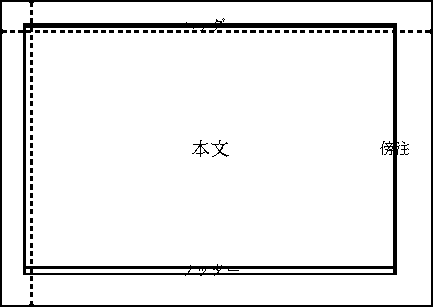
\includegraphics[scale=1]{geolay/geo11-1-crop.pdf}}%

%  vmargin=25mm,hmargin=15mm,
%  tmargin=25mm,bmargin=25mm,lmargin=15mm,rmargin=15mm,
%  top=25mm,bottom=25mm,left=15mm,right=15mm,

次は用紙サイズを A4 として,2段組,左右余白をそれぞれ 15\,mm,
上下余白を 25\,mm,段間の幅を 6\,mm,傍注・ヘッダー・フッター
なしの設定にします.

\GEO[\includegraphics]{a4paper,twocolumn,ignoreall,nomarginpar,noheadfoot,margin=\lb15mm\GQ25mm\rb,columnsep=6mm}{geolay/geo12-1-crop.pdf}{.3}{.7}
%\hbox{[scale=1]{geolay/geo12-1-crop.pdf}}%


\endinput
